\chapter{Diseño}

\section{Selección de herramientas}

\subsection{Sistema experto}

Para la implementación del sistema experto se consideraron las siguientes opciones:

\begin{itemize}

	\item \textbf{SWI-PROLOG}. Lenguaje basado en lógica y programación declarativa caracterizado por su capacidad de manipulación simbólica.

	\item \textbf{Expert System Builder}. Programa gratuito, implementado en Common Lisp, destinado a simplificar el desarrollo de sistemas expertos.

	\item \textbf{CLIPS}. Lenguaje basado reglas para desarrollar sistemas expertos. Basado en el lenguaje C para permitir una mayor portabilidad. 

\end{itemize} 

La herramienta Expert System Builder se desestimó al estar orientada al desarrollo de sistemas expertos para la toma de decisiones de una organización. 

La decisión entre escoger CLIPS o SWI-PROLOG se determinó por los siguientes factores:

\begin{itemize}

	\item CLIPS utiliza encadenamiento hacia delante y SWI-PROLOG encadenamiento hacia atrás. Los lenguajes que emplean encadenamiento hacia delante son más rápidos en el proceso de deducción, lo cuál hace que CLIPS sea más rápido en la ejecución de reglas que SWI-PROLOG.

	\item CLIPS se basa en el lenguaje C, el cuál sabemos es uno de los más eficientes en términos de velocidad computacional.

	\item Existen varias librerías para poder embeber sistemas expertos escritos en CLIPS en otros lenguajes como Java, Python o PHP.

\end{itemize} 

Por lo tanto, el sistema se implementará utilizando el lenguaje CLIPS.

\subsection{Interfaz}

La primera decisión que había que tomar sobre la interfaz era si diseñar una aplicación web o una aplicación de escritorio para comunicarse con el sistema experto. 

\bigskip
La aplicación de escritorio presenta las ventajas de ser más estable, robusta y eficiente en términos de velocidad.

\bigskip
La aplicación web presenta las ventajas de ser más accesible para los usuarios y una mayor portabilidad. Además, en caso de actualizar o mejorar el sistema, no habría ningún problema de incompatibilidad entre versiones. 

\bigskip
Debido a estas características, se optó por diseñar una aplicación web, principalmente por las ventajas que ofrece de portabilidad y actualización, dado que una de las ventajas de los sistemas expertos es su escalabilidad. 

\bigskip
 En un principio se optó por PHP, pero las librerías necesarias para poder implementar el sistema experto en PHP se encontraban desactualizadas, por lo que escogimos como herramienta utilizar un framework web de Python, \textit{DJango}. Se escogió Django de entre los posibles frameworks para web de Python por su gran comunidad y documentación más accesible y completa. Además, cuenta con una portente interfaz de administración y permite un desarrollo ágil y rápido.

 En las siguientes imágenes se muestra una idea inicial del diseño de las páginas de la interfaz:

 \begin{figure}[H]
 	\centering
	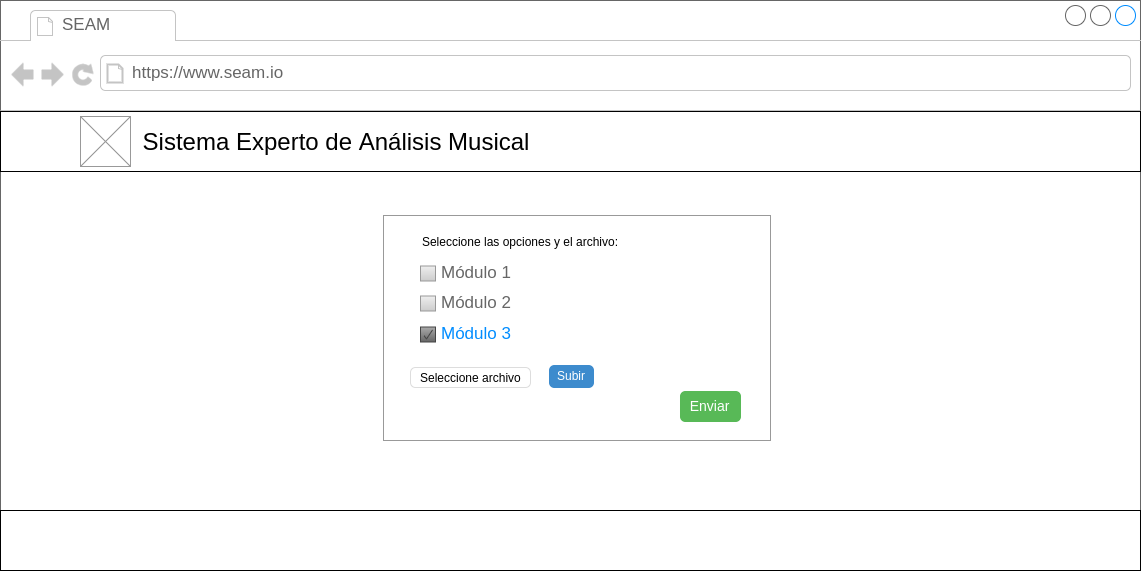
\includegraphics[scale=0.4]{imagenes/interfaz1.png}
	\caption{Wireframe de la página principal de la interfaz}
	\label{fig4.1.2.1}
\end{figure}

\begin{figure}[H]
	\centering
	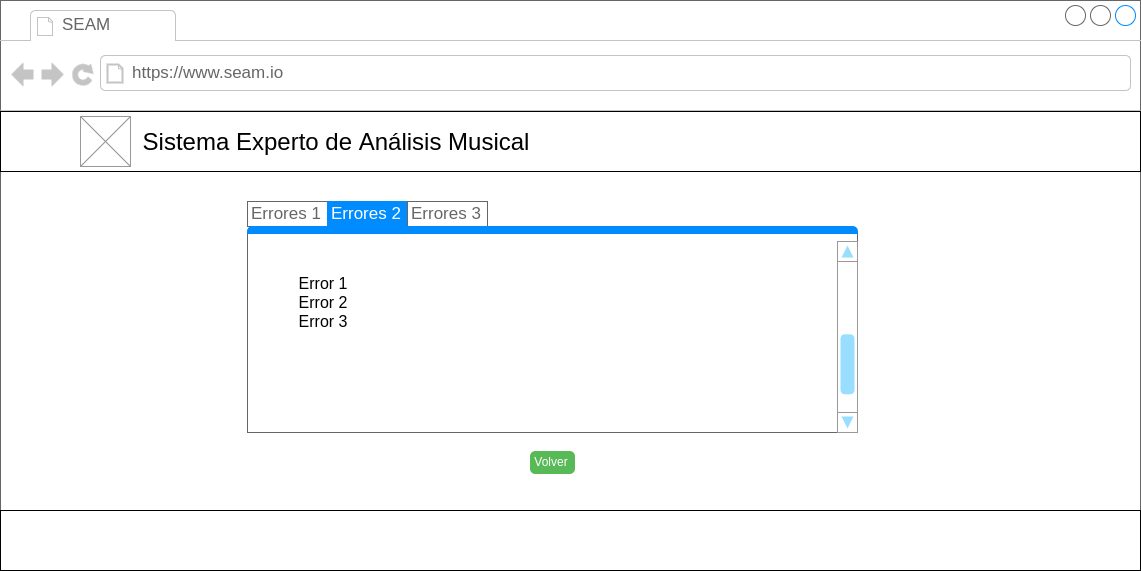
\includegraphics[scale=0.4]{imagenes/interfaz2.png}
	\caption{Wireframe de la página de resultados de la interfaz}
	\label{fig4.1.2.2}
\end{figure}

La maquetación de la interfaz se llevará a cabo haciendo uso de HTML5 y CSS3, apoyándonos en el sistema de temaplates Jinja2. Adicionalmente, se hará uso de jQuery para algunas funcionalidades.

\section{Arquitectura del sistema}

La arquitectura será \textbf{MVT} (Model-View-Template), que es la arquitectura empleada por DJango. En esta arquitectura, las vistas hacen el papel de ``controlador'' del sistema. Éstas serán las que contendrán al sistema experto.  

El sistema experto se dividirá en tres módulos:

\begin{itemize}

	\item Módulo 1: realizará la búsqueda de faltas en los acordes provocadas por los movimientos de las voces, como las faltas de quintas paralelas, octavas paralelas o duplicación de sensibles.

	\item Módulo 2: realizará el análisis melódico para señalar todos los errores en las líneas melódicas y su contrapunto.

	\item Módulo 3: comprobará la lógica tonal del coral y comprobará las secuencias de acordes, así como que estos se encuentren completos. 

\end{itemize}

En imagen \ref{fig4.2.1} se muestra gráficamente cómo sería la arquitectura del sistema.

\begin{figure}[H]
	\centering
	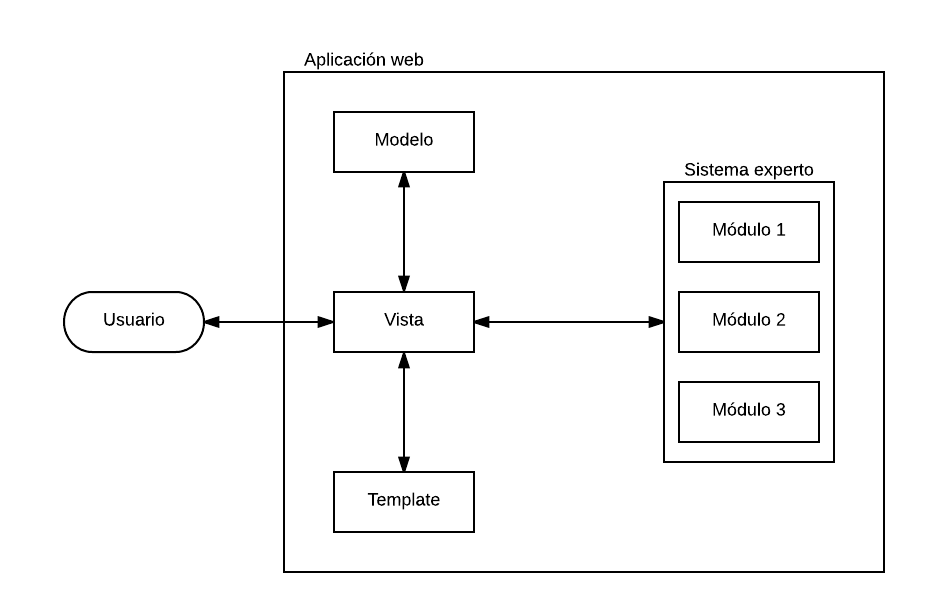
\includegraphics[scale=1]{imagenes/arquitectura.png}
	\caption{Diagrama de la arquitectura del sistema}
	\label{fig4.2.1}
\end{figure}